
\vspace{-0.1cm}
\section{Experiments}
\vspace{-0.2cm}

\begin{wrapfigure}{r}{.35\columnwidth}
\vspace{-0.3in}
\centering
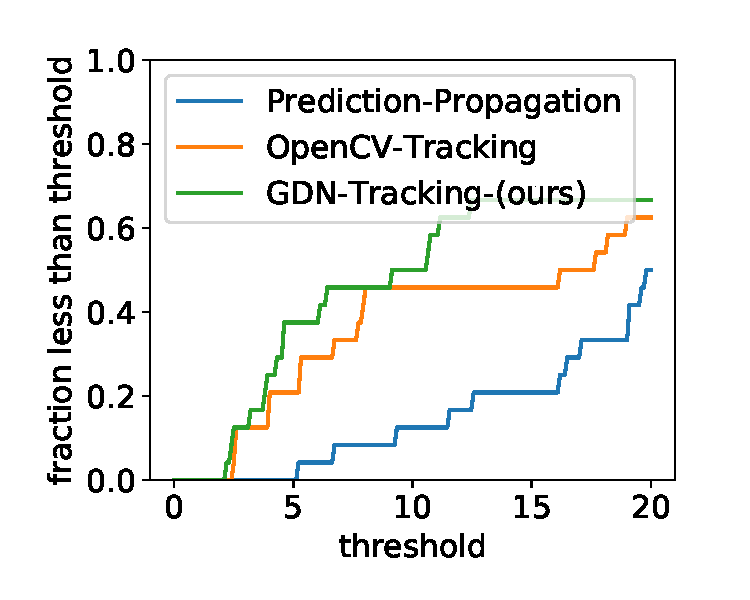
\includegraphics[width=0.35\columnwidth]{images/pushlong_bench_same_range.pdf}
\caption{\small{Real-world benchmark for pushing with 20 different tasks evaluated on unseen objects. Fraction of runs where final distance (in pixel units of 48x64 image) is lower than threshold. Our method shows a clear gain over OpenCV tracking and predictor propagation.}}
\label{fig:push_bench_long}
\vspace{-0.3in}
\end{wrapfigure}


Our experimental evaluation, conducted using two Rethink Sawyer robotic manipulators, evaluate the ability of our method to learn both prehensile and non-prehensile object relocation tasks entirely through autonomously collected data and self-supervision. In particular, we aim to answer the following questions: (1) How does our MPC approach with self-supervised goal image registration compare to alternative cost functions, such as off-the-shelf tracking and forward prediction via flow-based models? (2) When the robot can continuously retry a task with goal image registration, how much is the success rate for object relocation tasks improved? (3) Can we learn predictive models that enable both non-prehensile and prehensile object manipulation? We also present additional experimental comparisons in a simulated environment.
Videos and visualizations can be found on this webpage: \url{https://sites.google.com/view/robustness-via-retrying}.

\begin{wrapfigure}{r}{.35\columnwidth}
	\vspace{-0.3in}
	\centering
	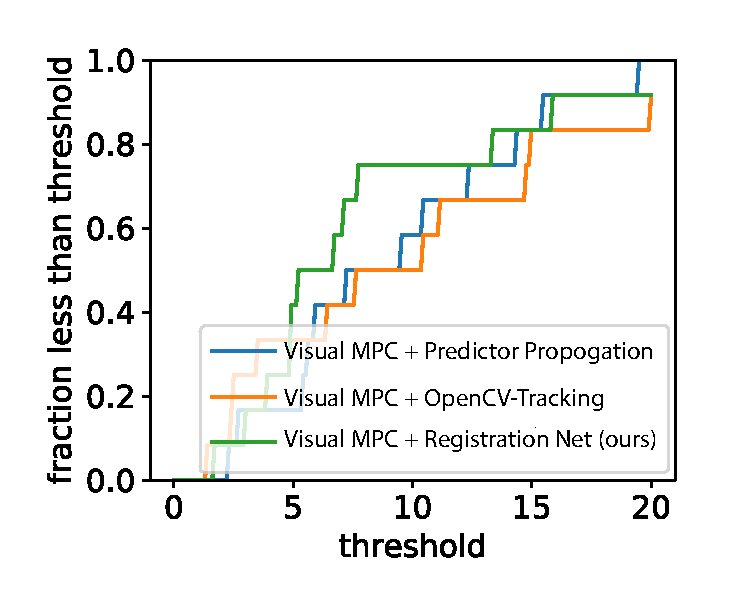
\includegraphics[width=0.35\columnwidth]{images/pushshort_bench_plots.pdf}
	\caption{\small{Benchmark for short distance pushing.  Fraction of runs where final distance is lower than threshold.}}
	\label{fig:push_bench_short}
%	\vspace{-0.3in}
\end{wrapfigure}

\subsection{Real-World Experiments}

To train both our prediction and registration models, we collected 20,000 trajectories of pushing motions and 15,000 trajectories with gripper control, where the robot was allowed to randomly move and pick up objects (we use objects 150 for training, 5 for testing, see the appendix for details). The data collection process is fully autonomous, requiring human intervention only to replace and change out the objects in front of the robot.
%%SL.06.15: would be nice to have a picture of data collection maybe?
The action space consisted of Cartesian movements along the $x$, $y$, and $z$ axes, and changes in azimuthal orientation of the gripper. For evaluation, we selected novel objects that were never seen during training. The evaluation tasks required the robot to move objects in its environment from a starting state to a goal configuration, and performance was evaluated by measuring the distance between the final object position and goal position. In all experiments, the maximum episode length was 50 time steps.

\vspace{-0.1in}
\paragraph{Pushing with retrying.}
\begin{figure}
    \centering
    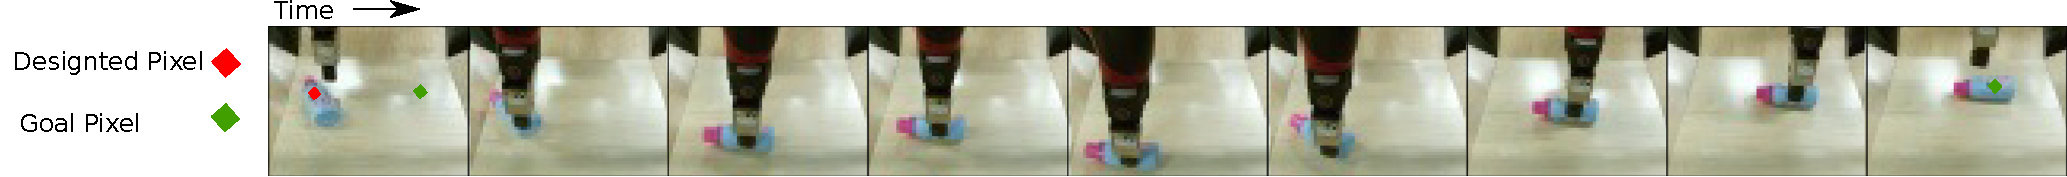
\includegraphics[width=1.0\textwidth]{images/push_correction.pdf}
    \caption{\small{Applying our method to a pushing task. In the first 3 time instants the object behaves unexpectedly, moving down. The tracking then allows the robot to retry, allowing it to eventually bring the object to the goal.}}
    \label{fig:push_retry}
\end{figure}

\begin{figure}
\vspace{-0.1in}
    \centering
    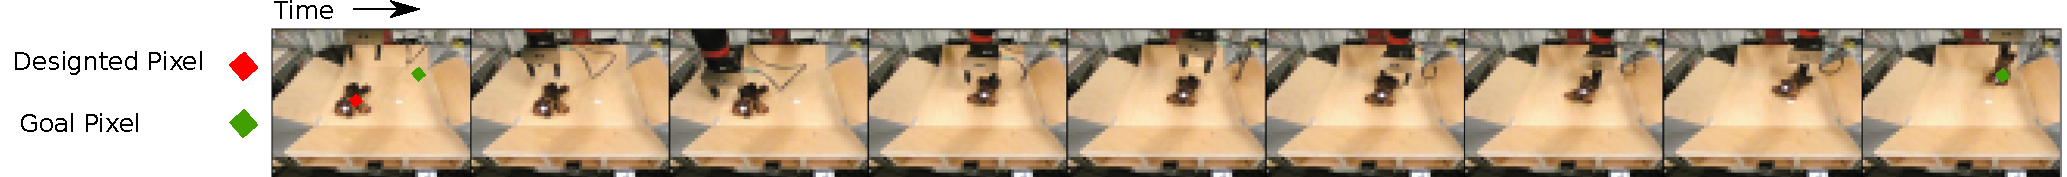
\includegraphics[width=1.0\textwidth]{images/pick_place_plush.pdf}
    \caption{\small{Retrying behaviour of our method combining prehensile and non-prehensile manipulation. In the first 4 time instants shown the agent pushes the object. It then loses the object, and decides to grasp it pulling it all the way to the goal. Retrying is enabled by applying the learned registration to both camera views (here we only show the front view).}}
    \label{fig:discrete}
    \vspace{-0.2in}
\end{figure}

In the first experiment, we aim to evaluate the performance of different visual MPC cost functions, including our proposed self-supervised registration cost. For this experiment, we disable the gripper control, which requires the robot to push objects to the target. 

We evaluate our method on 20 long-distance and 15 short-distance pushing tasks that require an object to be maneuvered to a target position. For comparisons, we include a baseline where the object is tracked using the ``multiple instance learning tracker'' MIL \cite{babenko2009visual} in OpenCV. 
%Note that our method does not have any prior knowledge of objects -- it is only provided with the position of one designed pixel in the initial and goal images, and must use the learned model to infer that this pixel belongs to an object that can be moved by the robot. 
We also compare to the visual MPC method proposed by \citet{sna},
%%SL.06.15: fill in citation
which does not track the object explicitly, but relies on the flow-based video prediction model to keep track of the designated pixel, which we call ``predictor propagation.'' 
%We also tested a method where the visual MPC cost is calculated by directly evaluating the error between the predicted image and goal image, but we found that this approach was unable to make meaningful progress in moving the object to the target. Instead it resulted in a policy that always moves the arm to the position indicted in the target image, as the arm accounts for the majority of the movable pixel mass in the image. This can be interpreted as undesirable local minimum which is not present in tracking based cost we propose.

\autoref{fig:push_bench_long} illustrates that on the long-distance benchmark our approach not only outperforms prior work \cite{sna}, but also outperforms the hand-designed object tracker \cite{babenko2009visual}. This is due to the fact that using our learned registration the agent is more frequently able to successfully recovering from situations where the object behaved differently than predicted the model predicted (see \autoref{fig:push_retry}). By contrast for short distance all methods perform comparably emphasizing the importance of c
%%SL.06.15: fill in discussion about what it does

\vspace{-0.1in}
\paragraph{Combined prehensile and non-prehensile manipulation.}

\begin{wrapfigure}{r}{.35\columnwidth}
\vspace{-0.3in}
\centering
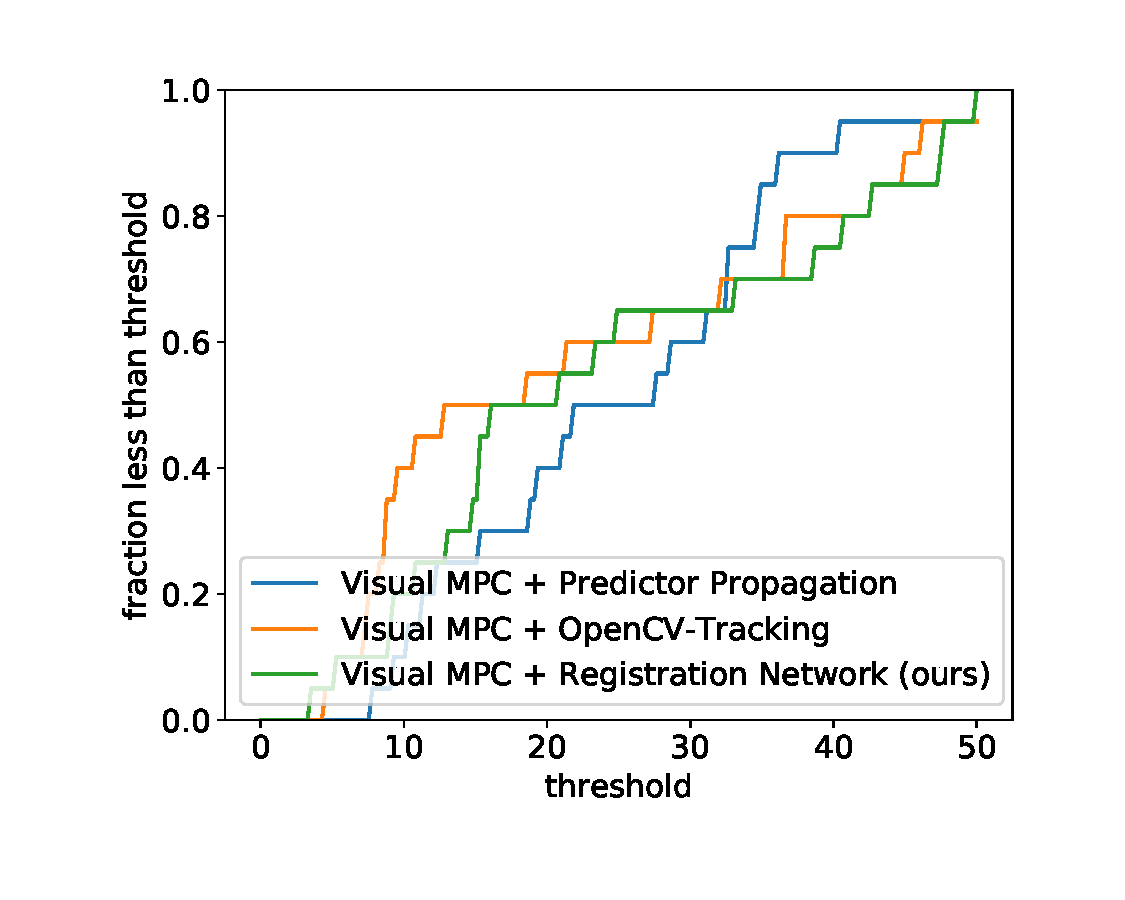
\includegraphics[width=0.35\columnwidth]{images/grasping_score_cdf.pdf}
\caption{\small{On the real-world grasping benchmark our method is on par with OpenCV tracking.}}
\label{fig:grasp_bench}
\vspace{-0.3in}
\end{wrapfigure}


In the setting where the gripper is enabled it is part of the task to decide whether to solve a task by prehensile or non-prehensile manipulation. Similarly to the pushing setting we perform a benchmark where we define a set of 20 object relocation tasks and measure the final distance between the object and the target at the end of the episode. Interestingly we observe that in the majority of the cases the agent decides to grasp the object, as can be seen in the supplementary video. \autoref{fig:grasp_bench} shows that the performance of our method is comparable with the performance of OpenCV tracking.


